\documentclass[11pt,a4paper]{article}

% ============================================================
% Comprobante de Registro OSF — CarniCore — Entrega 3 (2A)
% ISR-401 / 20303 — UTEQ
% ============================================================

\usepackage[utf8]{inputenc}
\usepackage[T1]{fontenc}
% Si el sistema tiene instalado texlive-lang-spanish, se puede activar:
% \usepackage[spanish]{babel}
\usepackage{geometry}
\geometry{a4paper, margin=2.5cm}
\usepackage{longtable}
\usepackage{booktabs}
\usepackage{array}
\usepackage{colortbl}
\usepackage{xcolor}
\usepackage{graphicx}
\usepackage{hyperref}
\usepackage{enumitem}
\usepackage{titlesec}
\usepackage{fancyhdr}
\usepackage{tabularx}
\usepackage{float}
\usepackage{framed}

% -------------------- Colores institucionales --------------------
\definecolor{uteqverde}{RGB}{0,90,60}
\definecolor{griscelda}{RGB}{240,240,240}

% -------------------- Encabezado y pie de página --------------------
\pagestyle{fancy}
\fancyhf{}
\renewcommand{\headrulewidth}{0.6pt}
\renewcommand{\footrulewidth}{0.4pt}
\lhead{\small UTEQ -- Ingeniería de Requerimientos (ISR-401 / 20303)}
\rhead{\small Comprobante de Registro OSF -- CarniCore -- Entrega 3 (2A)}
\cfoot{\thepage}

\hypersetup{
    colorlinks=true,
    linkcolor=uteqverde,
    urlcolor=uteqverde,
    citecolor=uteqverde,
    pdftitle={Comprobante de Registro OSF -- CarniCore -- Entrega 3 (2A)},
    pdfauthor={Equipo CarniCore -- UTEQ ISR-401},
}

\titleformat{\section}
  {\normalfont\Large\bfseries\color{uteqverde}}{\thesection}{1em}{}
\titleformat{\subsection}
  {\normalfont\large\bfseries}{\thesubsection}{1em}{}

% -------------------- Entorno para notas de cumplimiento --------------------
\newenvironment{notacumplimiento}
  {\begin{framed}\small\noindent\textbf{Nota de cumplimiento.}~}
  {\end{framed}}

\begin{document}

% ============================================================
% PORTADA / TÍTULO
% ============================================================
\begin{center}
    {\Large\bfseries Comprobante de Registro Previo en OSF}\\[0.3em]
    {\large Componente Empírico -- Sistema CarniCore -- Enfoque 2}\\[0.6em]
    {\small Ubicación en el repositorio: \texttt{06\_Experimento/osf\_registration.pdf}}
\end{center}

\vspace{0.5em}
\hrule
\vspace{1em}

% ============================================================
% DATOS DEL REGISTRO
% ============================================================
\section*{Datos del registro}

\renewcommand{\arraystretch}{1.4}
\begin{longtable}{@{}>{\bfseries}p{4.2cm} p{10.8cm}@{}}
\toprule
\rowcolor{griscelda}
Campo & Valor \\
\midrule
\endhead

Enlace persistente & \url{https://osf.io/wud69} \\
Fecha y hora de creación del proyecto & 02 de agosto de 2026, 1:12 AM \\
Fecha y hora de registro (\textit{Registered:}) & 02 de agosto de 2026, 12:31 PM \\
Título del registro &
Detección automática de ambigüedad en requisitos funcionales: un estudio de caso
en el dominio de trazabilidad cárnica (CarniCore) \newline
\textit{(asumido igual al título del protocolo; confirmar que coincide con el guardado en OSF)} \\
Plantilla de registro OSF &
Preregistration (formato con campos de \textit{Foreknowledge of data}, \textit{Starting
and stopping rules}, \textit{Indices}) \\
DOI &
No hay DOI asignado (confirmado en el panel lateral de OSF, campo ``Registro DOI'') \\
Licencia & CC0 1.0 Universal \\
Visibilidad & Privada \\
Protocolo adjunto &
\texttt{protocolo.pdf} (versión 1.0, 02/08/2026), consistente con el contenido del
formulario de registro \\
\bottomrule
\end{longtable}

% ============================================================
% VERIFICACIÓN DE PRECEDENCIA TEMPORAL
% ============================================================
\section*{Verificación de precedencia temporal}

Conforme al gatekeeper G6 de la Guía y Rúbrica de la Entrega 3 (2A), el registro debe
tener fecha anterior a toda recolección de datos (envío de la primera ficha de
clasificación experta y ejecución del detector).

El proyecto asociado se creó el 02/08/2026 a la 1:12 AM y el registro se completó ese
mismo día a las 12:31 PM. Ambos eventos son, por tanto, anteriores a cualquier
recolección de datos del componente empírico, que el equipo inicia únicamente después
de este registro, conforme al procedimiento de la Sección 8 del protocolo.

El propio formulario de registro declara explícitamente, en el campo
\textit{Foreknowledge of data or evidence}:

\begin{quote}
\itshape
``Data does not yet exist. No part of the data that will be used for this analysis
plan exists, and no part will be generated until after this plan is registered.''
\end{quote}

Esta declaración, hecha por el equipo al momento de registrar, constituye la evidencia
de precedencia temporal exigida por el gatekeeper.

% ============================================================
% CONSISTENCIA CON EL PROTOCOLO
% ============================================================
\section*{Consistencia con el protocolo}

Se verificó que el contenido del formulario de registro (preguntas de investigación,
hipótesis H0/H1, diseño censal sobre 25 RF, cegamiento y aleatorización con semilla
fija, métricas de precisión/\textit{recall}/F1/$\kappa$ de Cohen y Fleiss, software en
Python) es consistente con las Secciones 3, 4, 6, 9 y 10 de \texttt{protocolo.pdf}
versión 1.0. No se detectaron contradicciones entre ambos documentos.

% ============================================================
% CAPTURAS DE PANTALLA
% ============================================================
\section*{Captura de pantalla -- proyecto asociado}

% Reemplazar el bloque siguiente por:
%   \begin{figure}[H]
%       \centering
%       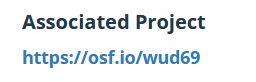
\includegraphics[width=0.6\textwidth]{figures/osf_proyecto_asociado.png}
%       \caption{Proyecto asociado en OSF.}
%   \end{figure}
\begin{figure}[H]
    \centering
    \fbox{\parbox[c][4cm][c]{0.7\textwidth}{\centering
        \textbf{Associated Project}\\[0.4em]
        \url{https://osf.io/wud69}\\[0.6em]
        \small [Insertar captura: \texttt{figures/osf\_proyecto\_asociado.png}]
    }}
\end{figure}

\section*{Captura de pantalla -- detalle del registro (privado)}

% Reemplazar el bloque siguiente por:
%   \begin{figure}[H]
%       \centering
%       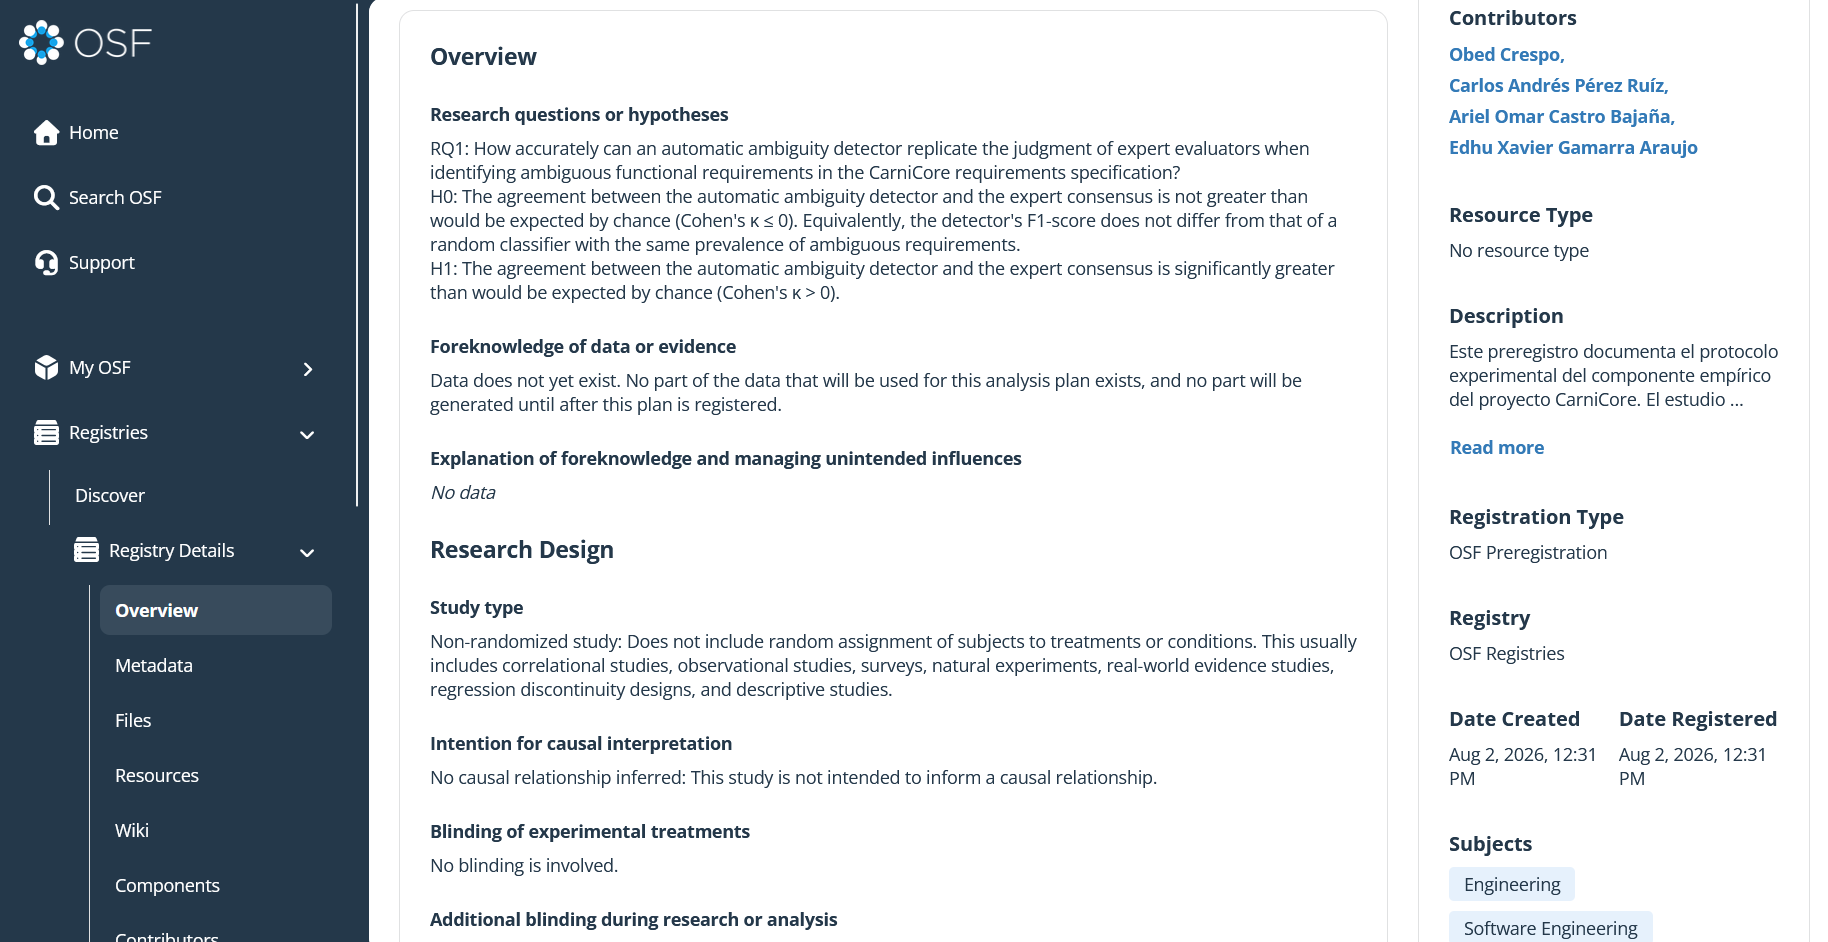
\includegraphics[width=\textwidth]{figures/osf_detalle_registro.png}
%       \caption{Detalle del registro OSF (visibilidad privada).}
%   \end{figure}
\begin{figure}[H]
    \centering
    \fbox{\parbox[c][6cm][c]{\textwidth}{\centering
        \small [Insertar captura: \texttt{figures/osf\_detalle\_registro.png}]\\
        (panel lateral con Proyecto Asociado, Licencia CC0 1.0 Universal y
        Registro DOI: \textit{No hay DOI})
    }}
\end{figure}

\noindent
Captura tomada desde la sesión autenticada del equipo (registro de visibilidad
privada), mostrando el panel lateral con el proyecto asociado
(\url{https://osf.io/wud69}), la licencia CC0 1.0 Universal y la confirmación de que
aún no hay DOI asignado.

\vspace{1em}
\begin{notacumplimiento}
Este comprobante documenta únicamente los datos confirmados directamente por el
equipo (enlace, fecha y hora de registro, visibilidad, licencia y estado del DOI) y
las capturas de pantalla correspondientes. No se completa ningún campo por
inferencia.
\end{notacumplimiento}

\end{document}
